% 
%  This file is included by Registration.tex
%

\begin{figure}
\center
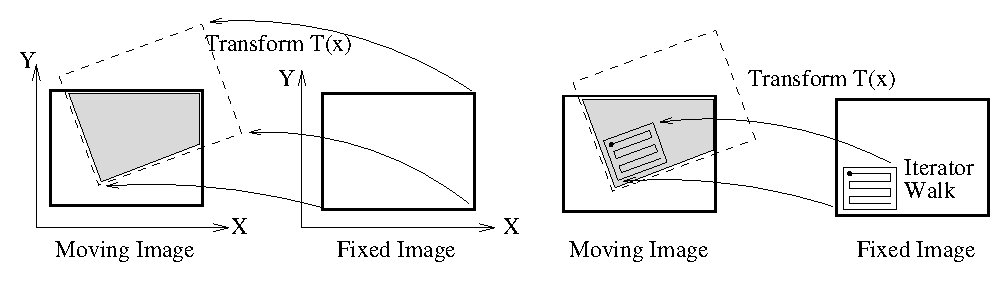
\includegraphics[width=16cm]{ImageOverlap.eps}
\caption{ The moving image is mapped into the fixed image space under some
spatial transformation. An Iterator walks throught the fixed image and its
coordinates are mapped onto the moving image.}
\label{fig:ImageOverlapIterator}
\end{figure}


\piccaption[2]{Grid positions of the fixed image map to non-grid positions of
  the moving image.\label{fig:ImageOverlapInterpolator}}
\parpic(8cm,6cm)[r]{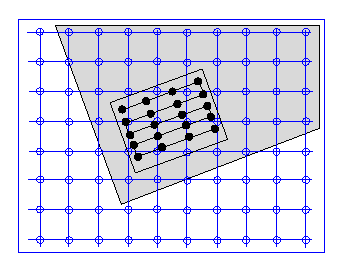
\includegraphics[width=7.5cm]{ImageOverlapInterpolator.eps}}

In the registration process, the metric typically compares intensity values 
in the fixed image with the corresponding values in the transformed moving
image. When a point is mapped from one space to another by a transform,
it will in general be mapped to a non-grid position. Therefore, interpolation
is required to evaluate the image intensity at the mapped position.

Figure \ref{fig:ImageOverlapIterator} (left) illustrates the mapping of the
fixed image space onto the moving image space. The transfom maps points from
the fixed image coordinate system onto the moving image coordinate system. The
figure highlights the region of overlap between the two images after the
mapping. The right side illustrates how an iterator is used to walk through a
region of the fixed image. Each one of the interator positions is mapped by the
transform onto the moving image space in order to find the homologous pixel.

Figure \ref{fig:ImageOverlapInterpolator} presents a detailed view of the
mapping from the fixed image to the moving image. In general the grid positions
of the fixed image will not be mapped onto grid positions of the moving image.
Interpolation is needed for estimating the intensity of the moving image at
these non-grid positions.


ITK currently offers three different interpolation schemes: nearest-neighbor,
linear and B-spline. In the context of registration, the interpolation method
affects the smoothness of the optimization search space and the overall
computation time. On the other hand, interpolations are executed thousands of
times in a single optimization cycle. Hence, the user has to tradeoff the
simplicity of computation with smoothness when selecting the interpolation 
scheme.

\index{itk::InterpolateImageFunction|textbf}
\index{itk::InterpolateImageFunction!SetInputImage()}
\index{itk::InterpolateImageFunction!Evaluate()}
\index{itk::InterpolateImageFunction!EvaluateAtContinuousIndex()}
\index{itk::InterpolateImageFunction!IsInsideBuffer()}

The basic input to a \code{itk::InterpolateImageFunction} is the image to
be interpolated. Once an image has been defined using \code{SetInputImage()},
a user can interpolate either at a point using \code{Evaluate()} or
an index using \code{EvaluateAtContinuousIndex()}.
 
Interpolators provide the method \code{IsInsideBuffer()} which tests whether a
particular image index or a physical point falls inside the spatial domain for
which image pixels exist.

\subsection{Nearest Neighbor Interpolation}
\label{sec:NearestNeighborInterpolation}
\index{itk::NearestNeighborInterpolateImageFunction|textbf}
\code{NearestNeigbhorInterpolateImageFunction} simply use the intensity of
the nearest grid position. That is, it assumes that the image intensity
is piecewise constant with jumps mid-way between grid positions. 
This interpolation scheme is cheap as it does not require any 
floating point computations.

\subsection{Linear Interpolation}
\label{sec:LinearInterpolation}
\index{itk::LinearInterpolateImageFunction|textbf}
\code{LinearInterpolateImageFunction} assumes that intensity varies linearly
between grid positions. Unlike nearest neighbor, the interpolated
intensity is spatially continuous. However, the intensity gradient
will be discontinous at grid positions.

\subsection{B-Spline Interpolation}
\label{sec:BSplineInterpolation}
\index{itkBSplineInterpolateImageFunction|textbf}
\code{BSplineInterpolateImageFunction} represents the image intensity 
using B-spline basis functions. When an input image is first 
connected to the interpolator, B-spline 
coefficients are computed using recursive filtering (assuming mirror
boundary conditions). Intensity at a non-grid position is computed
by multiplying the B-Spline coefficients with shifted B-Spline kernels
within a small support region of the requested position.

Currently, this interpolator support spline orders
from 0 to 5. Spline order of 0 is almost identical to nearest-neighbor;
spline order of 1 is exactly identical to linear interpolation. For 
spline order greater than 1, both the interpolated value and their
derivative are spatially continuous.

It is important to note that when using this scheme, the interpolated
value may lie outside the range of input image intensity. This is
especially important when handling unsigned data, as it is possible
that the interpolated value is negative.


